% !TeX root = ../Bachelorarbeit.tex
\chapter{Konzeption}
\section{Auswahl der Authentifizierungsverfahren}
\section{Prototypenaufbau}

\begin{center}
    \center
    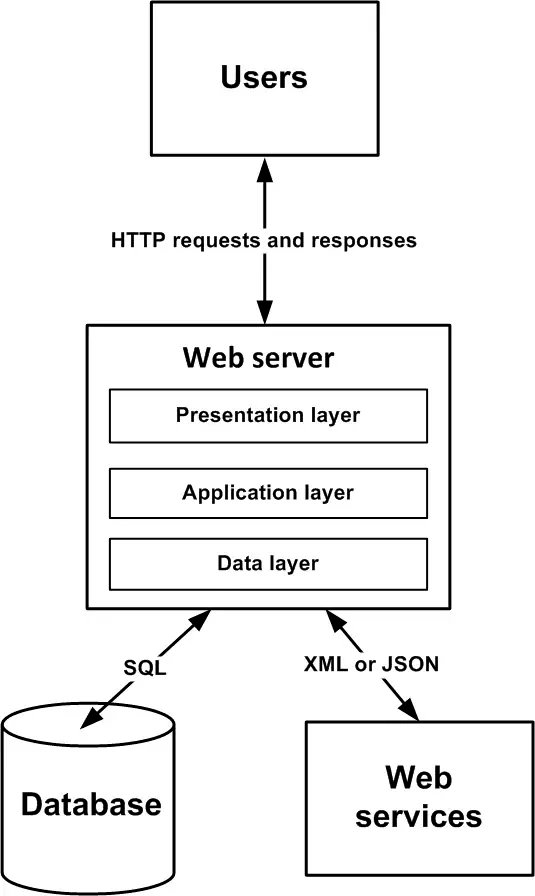
\includegraphics[width=10cm]{main-qimg-82af1fe49f85a31700d35570189a1fce.png}
\end{center} 

Das Ziel des Prototypen ist es, wie eingangs erwähnt, vorhandene Authentifizierungsverfahren abseits der klassischen UserID / Passwort Methode zu begutachten und dessen Schwächen aufzudecken. Daraus ergeben sich die typischen drei Komponenten von Drei-Tier-Client-Server Architekturen:

Ein Client, der Anfragen an die Applikation (das Backend bzw. den Server) sendet, welches die Daten dann in einer Datenbank mittels eines DBMS (Datenbankmanagementsystems) persistiert und verwaltet. Wie auch im Bild zur 3 Tier Architektur zu sehen, agiert der User auf dem Presentation Layer und stellt anfragen bzw. sendet JSON Objekte an den Server, der die entsprechenden Webservices liefert. Der Server speichert keine States, wodurch der Nutzer typischerweise mit jeder Anfrage alle benötigten Informationen liefern muss. Der Server liefert demnach lediglich die \ac{rest} Schnittstellen. Implementationsdetails und weitere Informationen zum Prototyp gibt es im nächsten Kapitel.
